\documentclass[11pt]{article}

\usepackage[margin=1in]{geometry}
\usepackage{graphicx}   % \includegraphics
\usepackage{booktabs}   % \toprule, \midrule, \bottomrule
\usepackage{caption}
\usepackage{hyperref}

\title{Sample Report: Random Forest vs.\ Other Binary Classifiers\\on the Ionosphere Dataset}
\author{Sample Student \\ COMP 395 -- Deep Learning}
\date{Fall 2026}

\begin{document}
\maketitle

\section*{Task and methods}

The UCI Ionosphere dataset contains 351 radar returns, each described by 34
numeric features and labeled \emph{good} (the signal shows structure in the
ionosphere) or \emph{bad}. It is close in size and difficulty to the breast
cancer data from Lab~2. I used a stratified 80/20 split (280 training and 71
test samples) and normalized every feature with the training mean and standard
deviation. I compared a random forest (200 trees) against five other methods:
the single sigmoid neuron from Lab~2 (MSE loss, SGD, $\alpha = 0.01$, 100
epochs), logistic regression, $k$-nearest neighbors ($k=5$), an RBF-kernel
SVM, and a single decision tree. All scikit-learn models used default settings.

\section*{Results}

Table~\ref{tab:results} and Figure~\ref{fig:accuracy} show that the random
forest and the SVM tied for the best test accuracy (95.8\%), followed by my
from-scratch neuron (94.4\%). Figure~\ref{fig:loss} shows the neuron's loss
falling quickly for about ten epochs and then flattening, so more epochs would
help very little.

\begin{table}[h]
  \centering
  \caption{Accuracy of each method. CV is the mean of 5-fold cross-validation
  on the training set (not run for the from-scratch neuron).}
  \label{tab:results}
  \begin{tabular}{lccc}
    \toprule
    Method & Train & Test & 5-fold CV \\
    \midrule
    Sigmoid neuron (from scratch) & 0.925 & 0.944 & --    \\
    Logistic regression           & 0.932 & 0.930 & 0.879 \\
    $k$-nearest neighbors ($k=5$) & 0.868 & 0.887 & 0.811 \\
    SVM (RBF kernel)              & 0.964 & \textbf{0.958} & \textbf{0.936} \\
    Decision tree                 & 1.000 & 0.901 & 0.875 \\
    Random forest (200 trees)     & 1.000 & \textbf{0.958} & 0.914 \\
    \bottomrule
  \end{tabular}
\end{table}

\section*{Discussion}

The two best models are the two that can draw curved decision boundaries,
which suggests the classes are not linearly separable; the linear models
(my neuron and logistic regression) land a few points lower. The single
decision tree memorized the training set (100\% train, 90.1\% test), a clear
sign of overfitting. The random forest also reaches 100\% on the training set,
but averaging 200 trees, each grown on a different bootstrap sample, cancels
much of that variance and recovers about six points of test accuracy.
$k$-NN did worst, probably because distances become less informative across
34 dimensions. One caution: with only 71 test samples, each sample is worth
1.4 percentage points, so the gap between the top three methods is one or two
radar returns. The cross-validation column is the steadier comparison, and
there the SVM leads the random forest by about two points.

\begin{figure}[h]
  \centering
  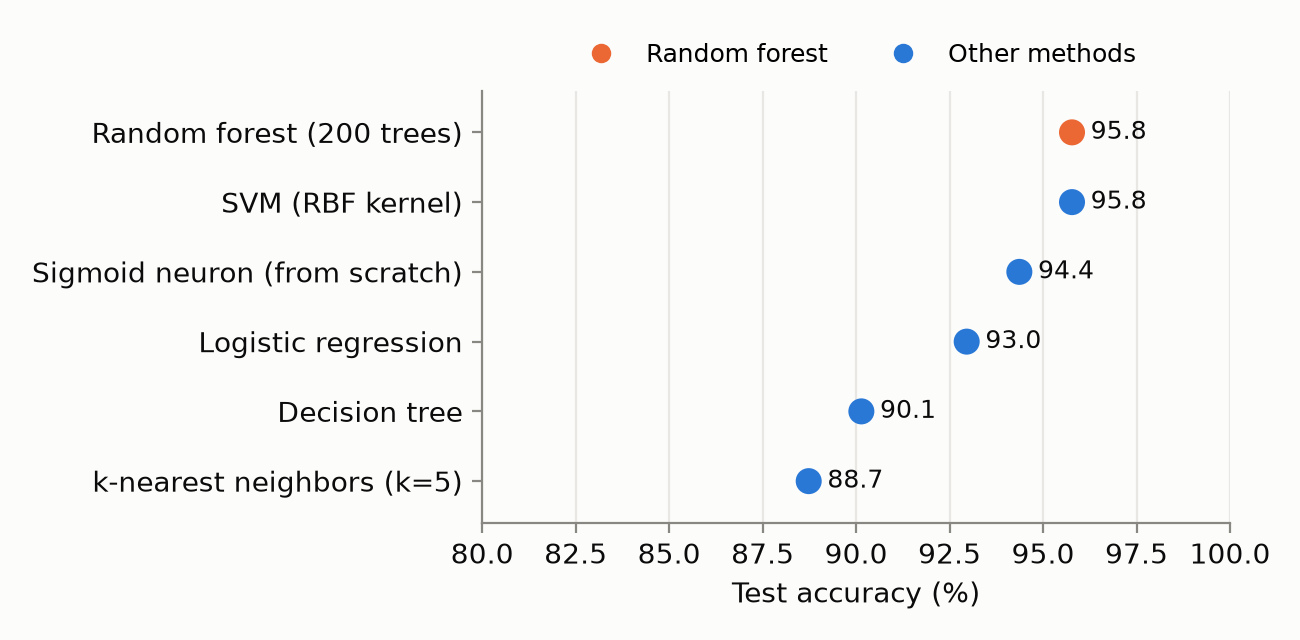
\includegraphics[width=0.85\textwidth]{accuracy_comparison.png}
  \caption{Test accuracy of each method (71 test samples).}
  \label{fig:accuracy}
\end{figure}

\begin{figure}[h]
  \centering
  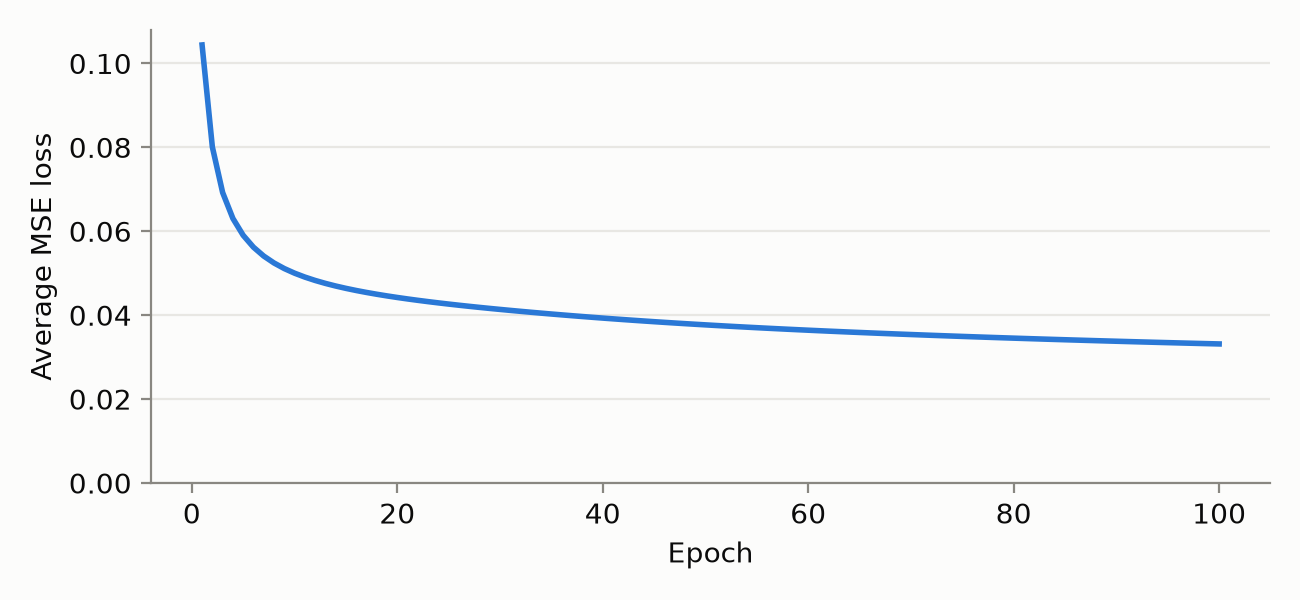
\includegraphics[width=0.8\textwidth]{training_loss.png}
  \caption{Average training loss per epoch for the from-scratch sigmoid neuron.}
  \label{fig:loss}
\end{figure}

\end{document}
